\section{Beyond graphene: TMD nanoribbons}
\label{sec:state}

Planar materials have steadily been drawing the attention of the community since graphene was isolated from a graphite sample by mechanical exfoliation \cite{novoselov_electric_2004}(Fig.(\ref{fig:graphene}), left).
Since then, numerous studies have been made concerning the interesting as-yet-unseen phenomena occurring within these materials. For example, in the case of graphene, we have: unconventional quantum Hall effect, absence of localization, and electrons behaving like massless relativistic particles at low energies (Fig.(\ref{fig:graphene}), right), providing a bridge between condensed matter physics and quantum electrodynamics \cite{katsnelson_graphene:_2007}.
In spite of its undeniable potential both from a fundamental and an application point of view, graphene has some shortcomings.
This motivated the community to study other more complex graphene-like materials, which could have other desirable properties, while maintaining most of graphene's potential.
\begin{figure}[H]
\hspace{2.5cm}

\includegraphics[width = 2.3cm]{Introduction/graphene.png}
\hspace{3.5cm}
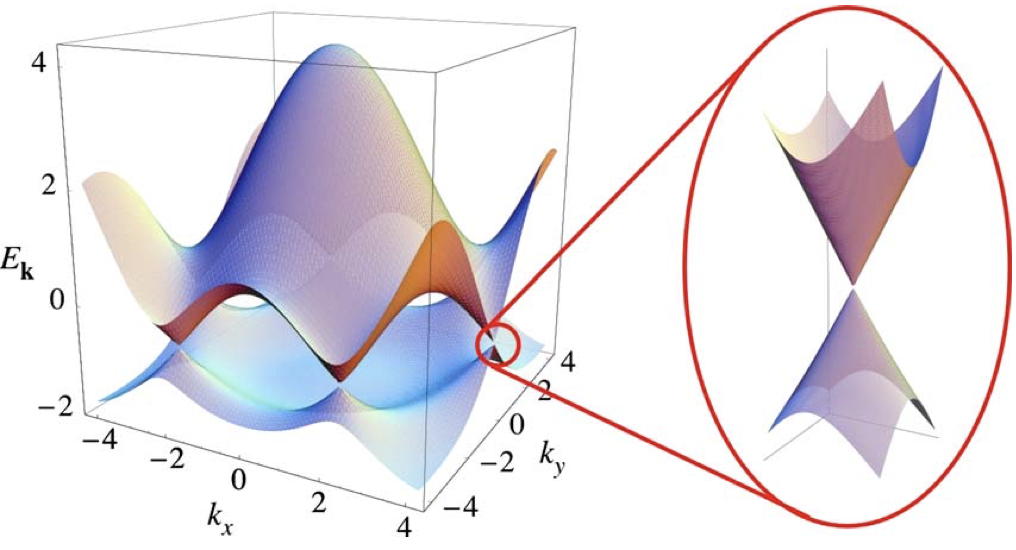
\includegraphics[width = 6.3cm]{Introduction/dispGraphene.png}
\caption[Graphene monolayer; graphene's dispersion relation.]{Left: \acf{AFM} picture of a graphene monolayer. The black area is a substrate used for fabrication purposes. The dark orange area is a monolayer of graphene. Right: Dispersion relation of graphene.
Close to the charge neutrality point, the dispersion relation is linear, corresponding to massless excitations (taken from \cite{castro_neto_electronic_2009}). }
\label{fig:graphene}
\end{figure}	

\acl{TMD}s are prominent examples of such novel members of the \ac{2D} materials family \cite{wang_electronics_2012, roldan_electronic_2014, xu_spin_2014}.
An excellent review of their properties, experimental results and applications is given in \cite{manzeli_2d_2017}.
Much like graphite which is essentially constituted by stacked monolayers of carbon atoms bound by weak Van der Waals forces, 3D \ac{TMD} structures are also formed by weakly bound layers.
However, instead of carbon, the layers contain transition metals $M$, and chalcogens $X$, in a $1-2$ proportion.
Thus, group 6 \acp{TMD} are denoted $MX_2$, where $M = \text{Mo}, \text{W}, ...$ (respectively Molybdenum and Tungsten) and $X = \text{S}, \text{Se}, \text{Te}$ (respectively Sulfur, Selenium and Tellurium).
Each \acs{TMD} monolayer contains a layer of $M$ atoms organized in a triangular lattice sandwiched between two layers of $X$ atoms,unlike graphene( where carbon atoms are all on the same plane).
Each $M$ atom is coordinated with six $X$ atoms, in a stacked structure with various possible coordinations for the $X$ atoms.
The most common phases are trigonal prismatic (2H) and octahedral (1T), typically in the few $\angstrom$ range (for Molybdenum disulfide, $\text{Mo}\text{S}_2$, the width is around $6.5 \angstrom$).
Therefore, for our purposes, we shall take a $2H$ configuration seen as a planar honeycomb lattice, as depicted in the top-down view of Fig (\ref{fig:tmdHex}a).
In these lattice models, the valence bands arise out of the hybridization of the $d_{xy}$ and $d_{x^2 - y^2}$ orbitals of the transition metal with the $p_{x, y}$ orbitals of the chalcogen, while conduction bands have a main contribution from the $d_{3z^2 - r^2}$ orbitals of the $M$ atoms with only a minor contribution from the $p_{x, y}$ orbitals of the $X$ atoms.
%revise english
\begin{figure}[H]
\centering
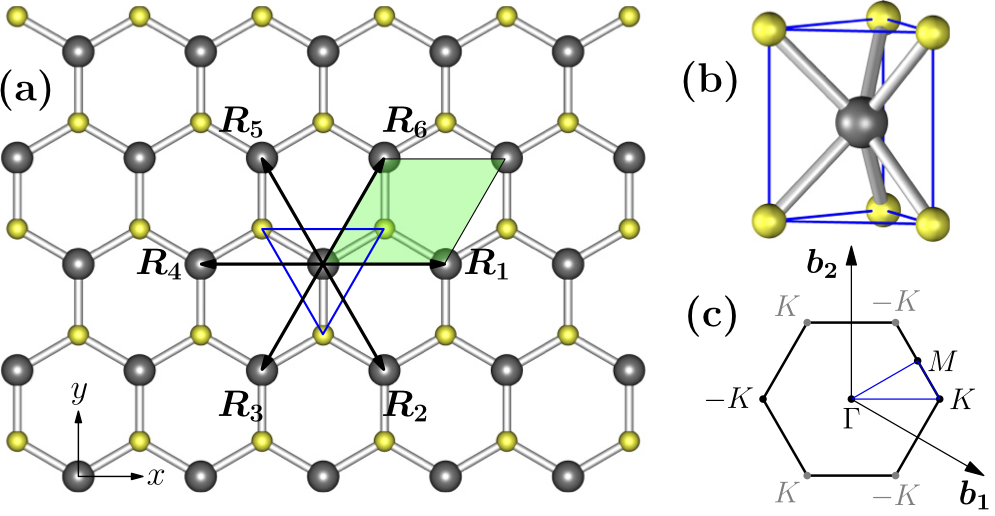
\includegraphics[scale = 0.23]{Introduction/tmd2.png}
 \caption[\ac{TMD} monolayer condensing in its 2H phase.
 $M-X$ honeycomb lattice.
 Unit cell of the trigonal prismatic (2H) phase of a \ac{TMD} monolayer.
 High symmetry points of the corresponding hexagonal lattice's  reciprocal space.]{(a) The 2H phase of a  \ac{TMD} monolayer may be viewed simply as a $M-X$ honeycomb lattice. Here we represent the six nearest neighbors of a point on the $M$ triangular lattice by the real space vectors $\bm R_{i = 1,2,..., 6}$.
(b) Unit cell of the trigonal prismatic (2H) phase of a \ac{TMD} monolayer.
(c) High symmetry points $\Gamma, M, K$ of the first Brillouin zone ($\bm b_{1,2}$ are the reciprocal basis vectors).\label{fig:tmdHex}}
\end{figure}

\acl{2D} \acp{TMD} have been attracting interest because they seem to overcome some of the drawbacks of graphene in technological applications.
For example, monolayer graphene is gapless, while its bilayer counterpart has a tunable, but small gap of the order of a tenth of an $eV$.
Contrastingly, monolayer \acp{TMD} are semiconductors, having an intrinsic gap in excess of $1 \, eV$, which lies at the inequivalent $K$ points of the hexagonal Brillouin zone.
Thus, \acp{TMD} are more promising for designing, for example, transistors.
More generally, since the direct band gap lies in the visible frequency range, and room temperature mobility is good, these semiconducting analogues of graphene are promising for electronic and optoelectronic applications.
Perhaps even more striking is the appearance of an extra so called \emph{valley} degree of freedom.
Since the valence and conduction band edges both lie at the two corners ($\pm K$) of the first Brillouin zone, electrons and holes can acquire an extra degree of freedom which can be used to encode and process information.
Additionally, the presence of giant spin-orbit coupling and the lack of inversion symmetry lead to a strong coupling between valley and spin, suggesting that \acp{TMD} could allow the integration of spintronics and valleytronics, yielding a greater control of electron systems through their coupled spin and valley degrees of freedom, analogously to what is done in electronics, where only the charge degree of freedom is used.
 
Hole-doped \acp{TMD} are expected to show topological superconductivity \cite{hsu_topological_2017}, while the superconducting phase of graphene has been predicted, but is not easily attained.
Superconductivity in graphene-like \ac{2D} materials is important because it could boost high speed nanoelectronics.
Moreover, the presence of transition metal atoms in \acp{TMD} suggests the possibility of magnetic ordering \cite{braz_valley_2017}, which could be very relevant in nanospintronics applications.
Both superconductivity and magnetic ordering may arise due to the effect of strong electron correlations.
Thus, to investigate these properties of \acp{TMD} reliably, we need a computational method that can  capture the effects of strong electron-electron interactions accurately.
As we shall see, auxiliary field \ac{QMC}  fulfills this criterion.

\subsection{Electronic properties}\label{subsec:electronic}

The electronic properties of \ac{TMD} monolayers depend crucially on $\text{X}$-coordination.
In particular, for the 2H phase, they may ultimately be attributed to the lack of inversion symmetry relative to the $M$ atoms.
This leads to the spin splitting of the electronic bands driven by spin-orbit coupling.
%Because $K$ and $K'$ (or $-K$) no longer correspond to time reversal invariant momenta, the spin degeneracy of the valence and conduction bands is lifted at these points.
Time-reversal symmetry implies that the splitting is opposite at the $K$ and $K'$ points, leading to the band structure of Fig. (\ref{fig:tmdProp}d) (we show the part relevant for realistic charge-carrier concentrations).
This property, known as spin-valley coupling, implies that the valley polarization of charge carriers directly translates into spin polarization, leading to an intrinsic property of \acp{TMD} that could allow the design of spintronic devices without resorting to magnetic materials \cite{manzeli_2d_2017}.
More broadly, the possibilities afforded by the different compositions and structural phases listed in Fig.(\ref{fig:tmdProp}) lead to a vast array of electronic properties.
On the one hand, the band structure and its metallic/insulating character vary quite substantially among \acp{TMD}.
On the other hand, both highly nontrivial  correlated and topological phases arise within these materials.
In this work, we investigate the properties of correlated phases in zigzag edged \ac{TMD} nanoribbons.
\begin{figure}
\centering
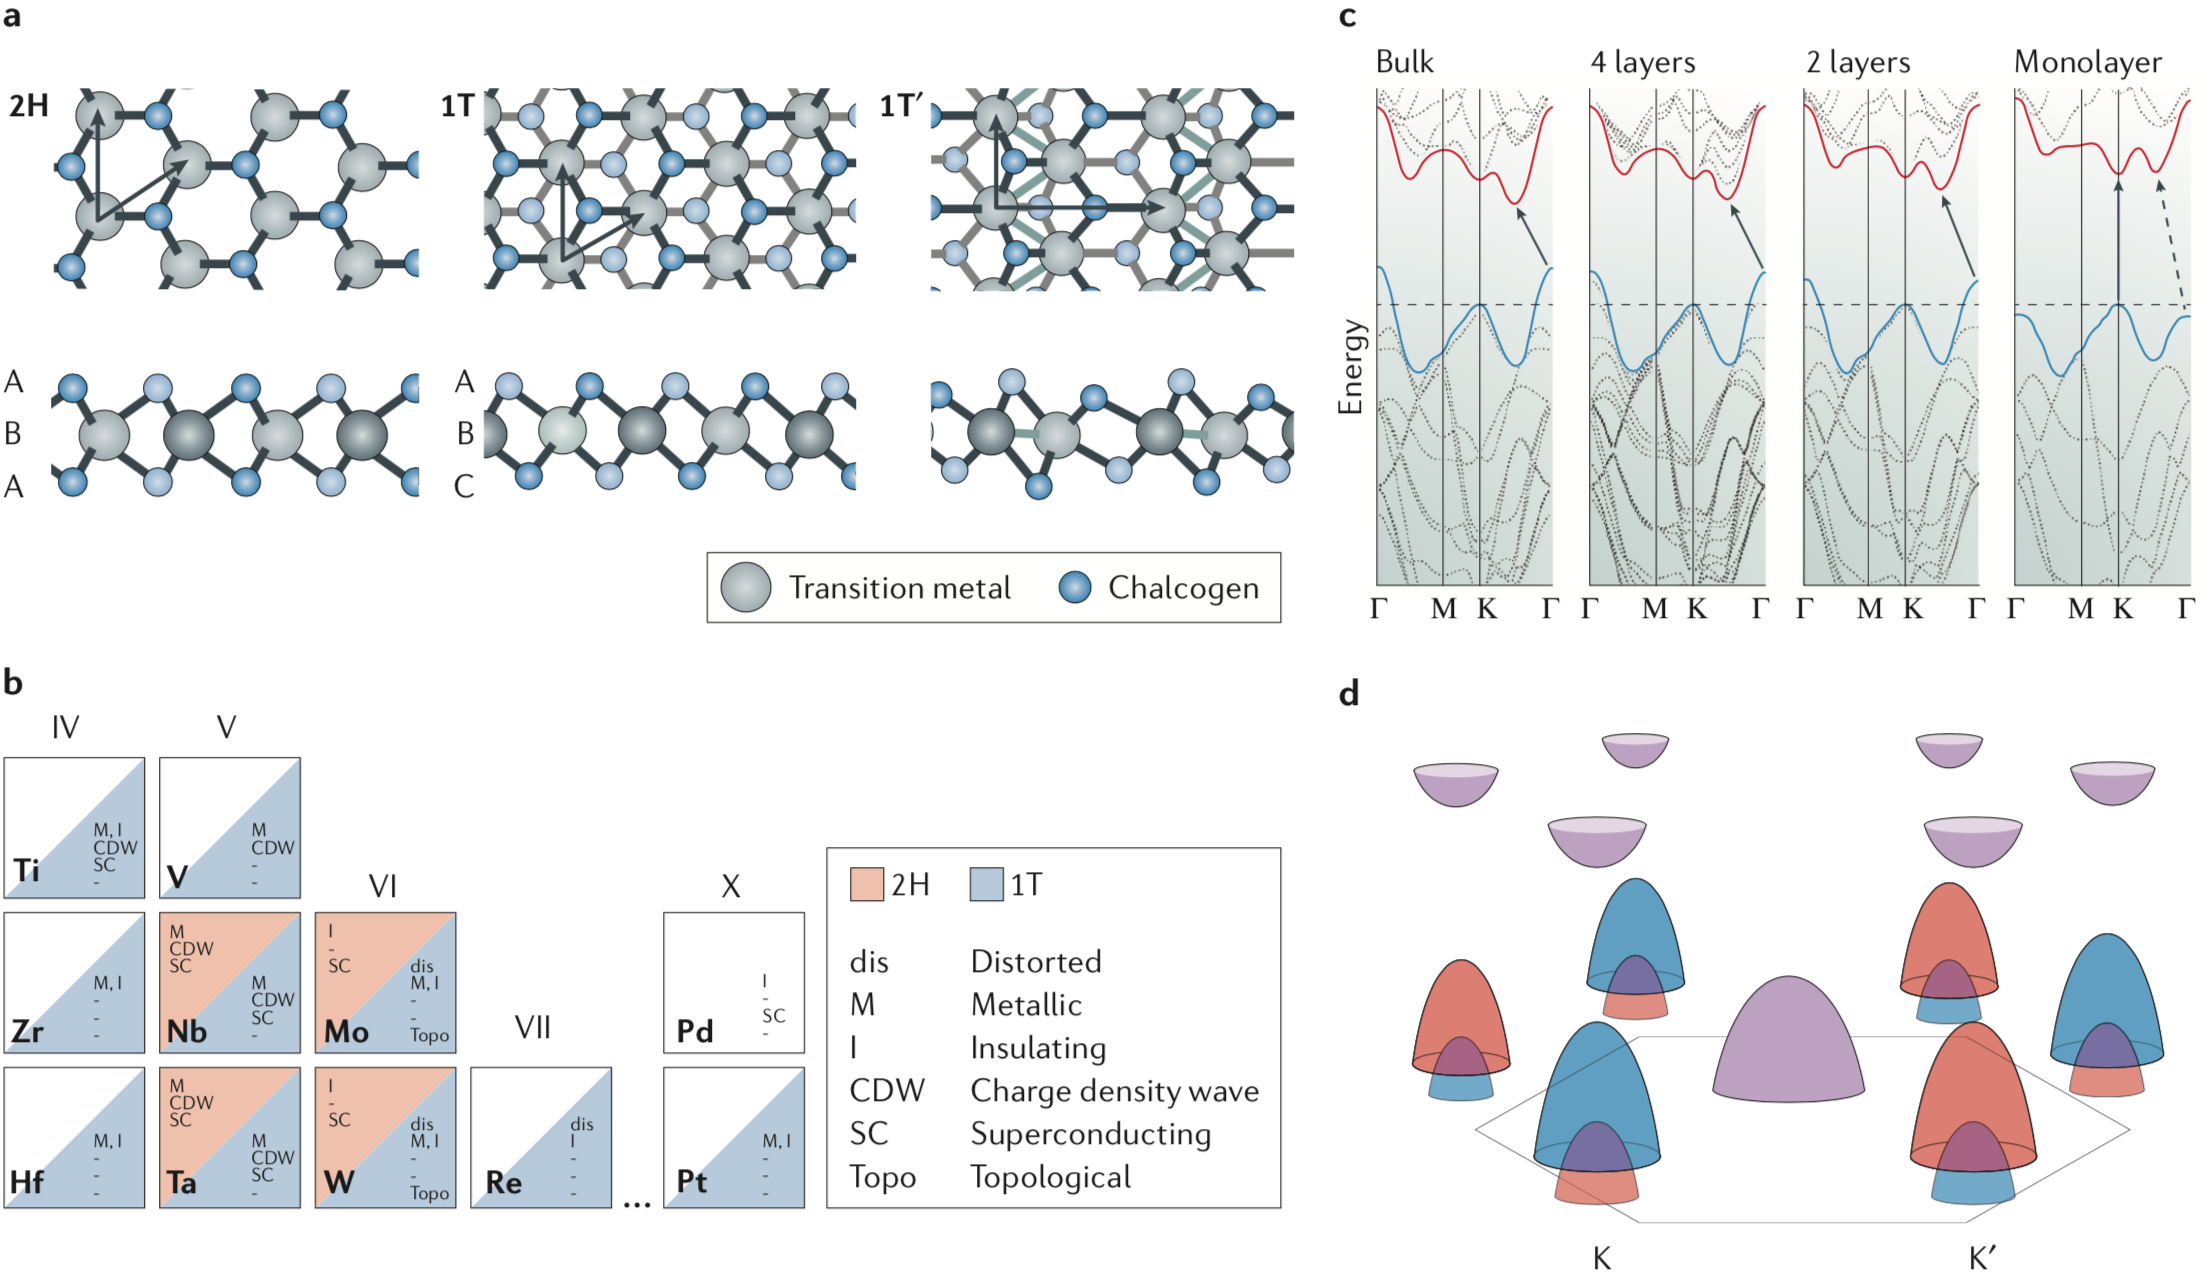
\includegraphics[scale = 0.37]{Introduction/tmdProp}
 \caption[Structure and electronic properties of \ac{TMD} monolayers.]{(a) Some of the possible structural phases of \ac{TMD} monolayers: trigonal prismatic (2H) with ABA stacking, distorted octahedral (1T), and dimerized octahedral (1T'), showing ABC stacking. (b) A periodic table of known \ac{TMD} layers. Shown are the transition metals involved, the existing phases (2H and/or 1T), and the possible electronic phases. (c) Calculated band structure (from density functional theory \cite{splendiani_emerging_2010}) of $2H-\text{Mo}\text{S}_2$ for samples of decreasing thickness. (d) Representation of the band structure of monolayer $2H-\text{Mo}\text{S}_2$, showing the spin splitting (red for spin-up, blue for spin-down) of the bands near the corners of the Brillouin zone (K and K'). \label{fig:tmdProp}}
\end{figure}

\subsection{Nanoribbons}\label{subsec:nanoribbons}

Nanoribbons are a particularly promising type of \acs{2D} nanostructure.
They consist of \ac{2D} layers that can be regarded as infinitely long on one direction, but not on the other (Fig.(\ref{fig:graphNanoFabricationTMD})), so that the edge-states become relevant in their physical properties.
For simulation purposes, we assume translational invariance along the ribbon's longitudinal direction, by the use of \acp{PBC}.
On the transverse direction, we use \acp{OBC},  considering zigzag edges (see Fig.(\ref{fig:nanoribbons_energiesTMDs}), left).
\begin{figure}[H]
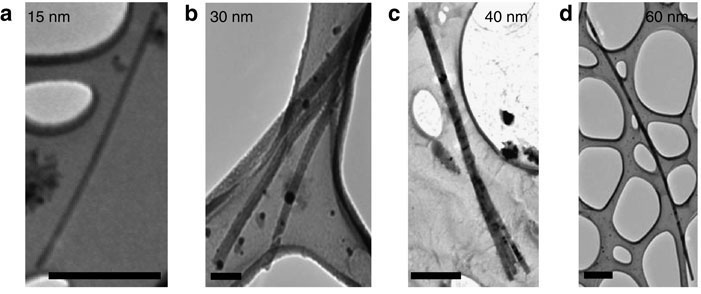
\includegraphics[scale = 0.233]{Introduction/grapheneNanoribbons.jpg}
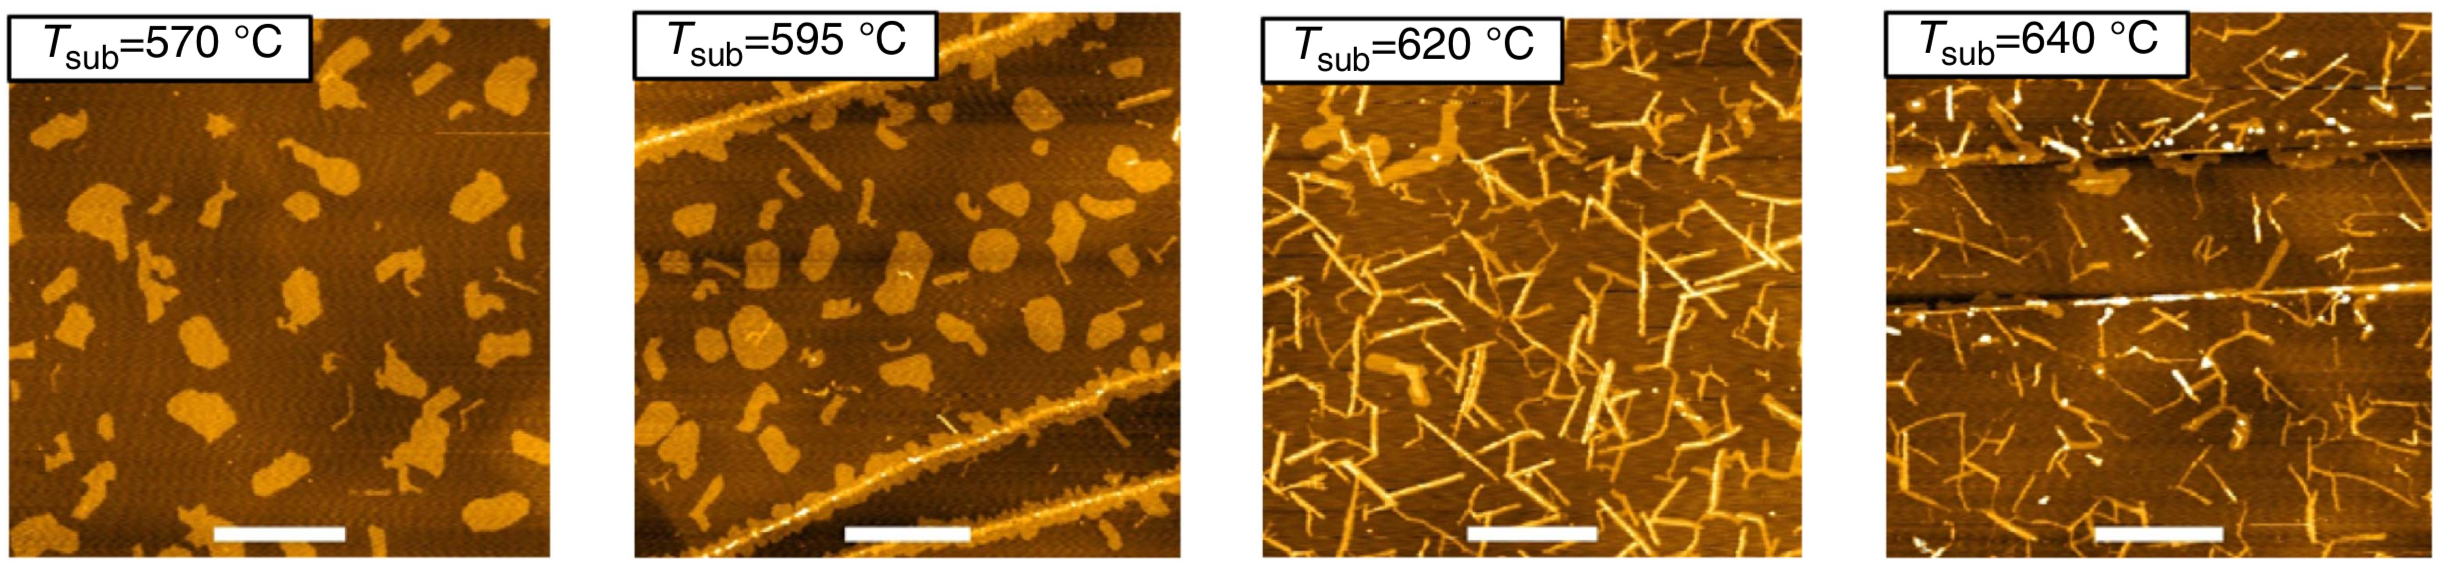
\includegraphics[scale = 0.233]{Introduction/nanoribbons}
\caption[(TEM) images of graphene nanoribbons. Fabrication of \ac{TMD} nanoribbons.]{Left: (a) to (d) - Transmission electron microscopy (TEM) images of graphene nanoribbons (GNRs) of widths 15, 30, 40, and 60 $nm$ (adapted from \cite{mohanty_nanotomy-based_2012}). Right: Fabrication of \ac{TMD} nanoribbons. Left to right: \ac{AFM} images showing the appeareance of nanostructures ranging from \ac{2D} nanoislands to nanoribbons, as the temperature of the substrate is increased. The nanoribbons are grown by taking advantage of the temperature dependence of shape transformations occuring during the nonequilibrium growth of surface-based nanostructures (taken from \cite{chen_fabrication_2017})}
\label{fig:graphNanoFabricationTMD}
\end{figure}

Ab initio calculations indicate that a large density of low-energy electronic states is localized at the zigzag edges, decaying quickly in the bulk, which suggests the possibility of magnetic ordering.
In fact, a mean field solution of the Hubbard model for a graphene nanoribbon shows that magnetic moments are localized at the edges \cite{yazyev_emergence_2010} (see Fig.(\ref{fig:nanoribbons_energiesTMDs}), left).
QMC has been used to investigate edge-state magnetism beyond mean field in graphene \cite{feldner_dynamical_2011, golor_quantum_2013, cheng_strain-induced_2015, raczkowski_interplay_2017, yang_strain-tuning_2017}.
However, edge-state magnetism in zigzag-edged \ac{TMD} nanoribbons remains unexplored \cite{davelou_nanoribbon_2017}, and we would like to investigate, for example, whether edge-state magnetism is stabilized at finite temperature in such systems, following the tendency that was identified for their graphene counterparts.
While the zigzag graphene nanoribbon antiferromagnetic ground state is semiconducting, a state with interedge ferromagnetic orientation is a metal.
An example of an application based on the switching between the two states is a magnetorresistive sensor.
This device allows switching between low and high-resistance configurations, corresponding, respectively, to parallel, and antiparallel configurations of ferromagnetic leads at the ends of a nanoribbon.
An analogous form of edge-state magnetism, as is observed in graphene nanoribbons, for \acp{TMDNR}, could yield similarly innovative applications.
\begin{figure}[H]
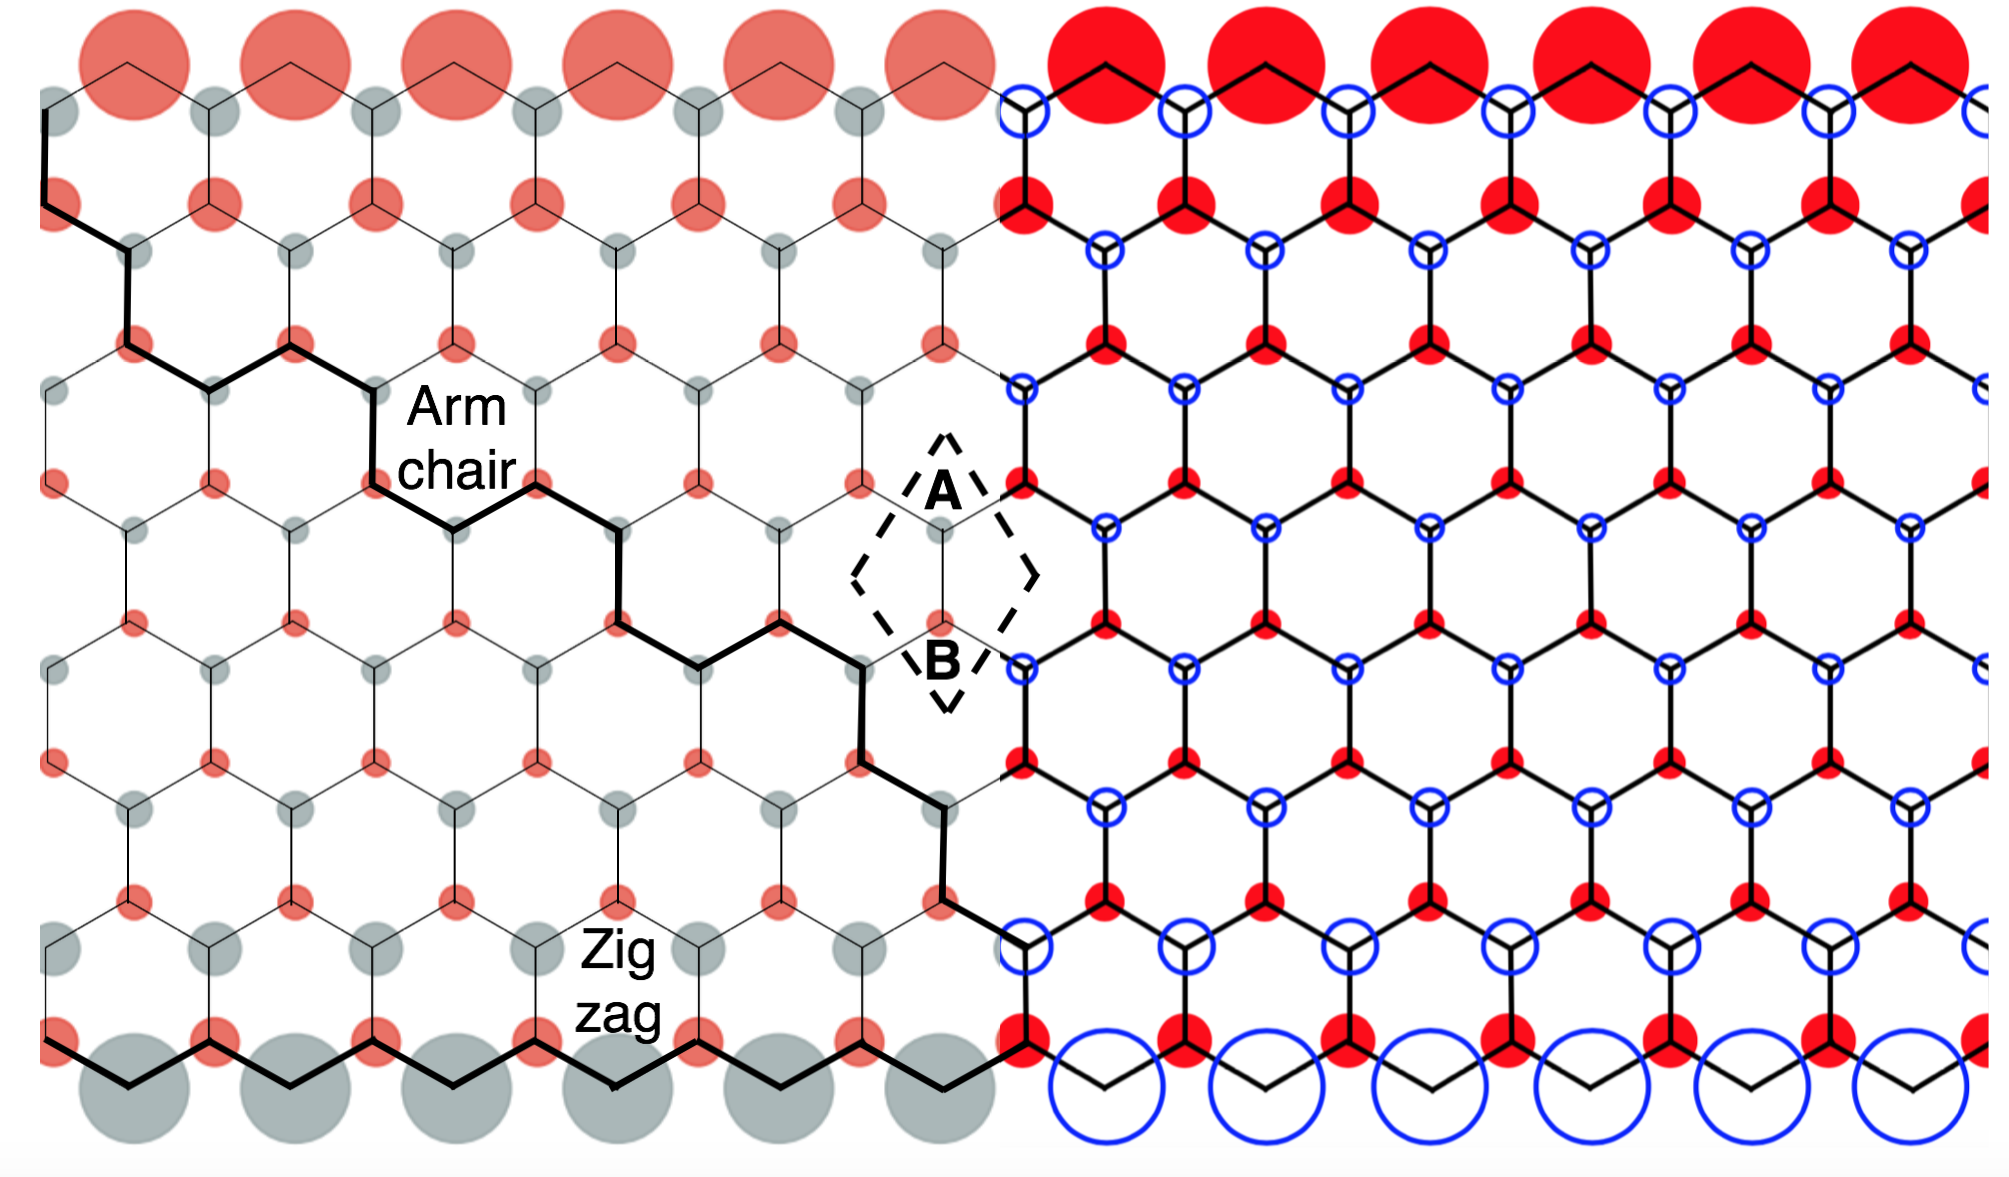
\includegraphics[scale=0.225]{Introduction/comparisonMF_edges}
\hspace{5mm}
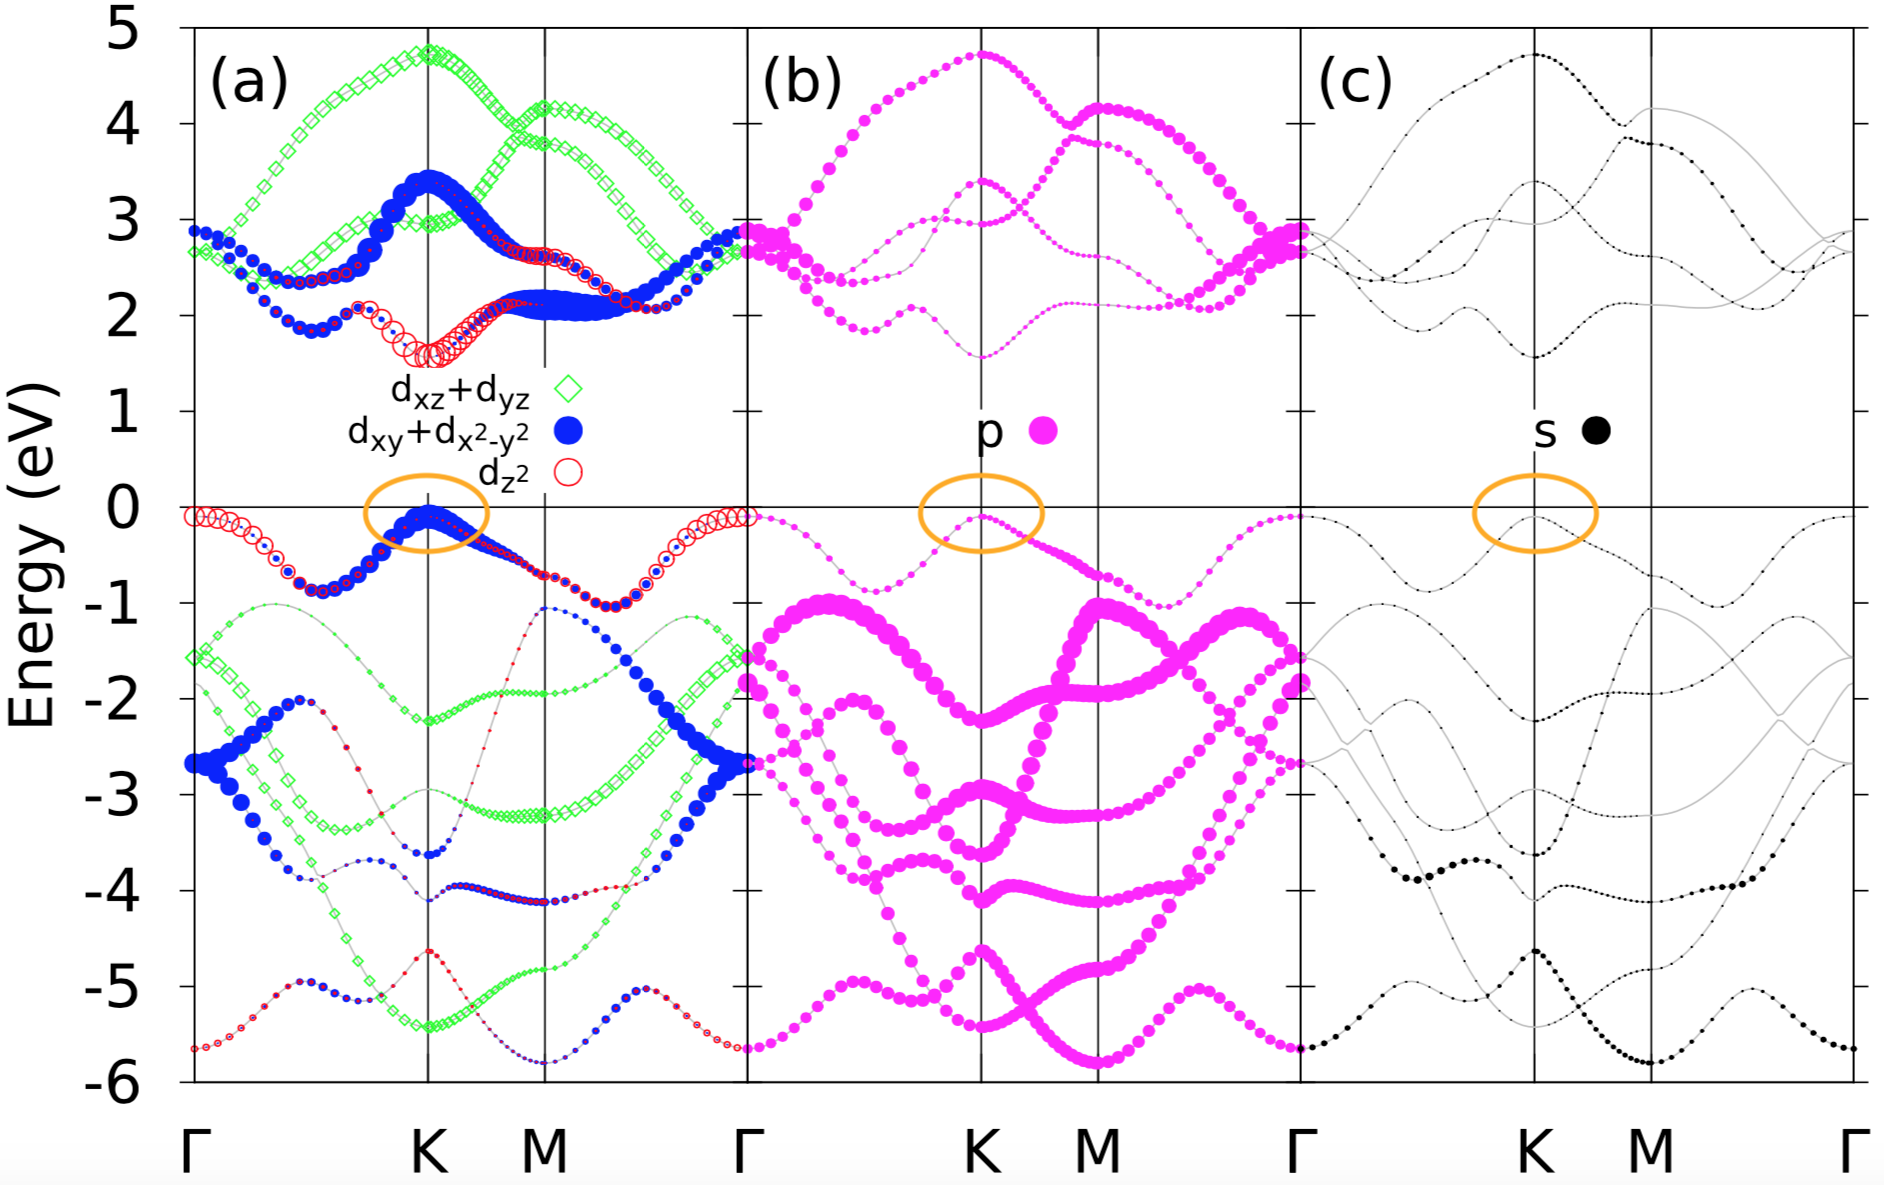
\includegraphics[width = 7.22cm]{Introduction/energiesTMDs}
 \caption[Zigzag edges of a nanoribbon and magnetism. Orbital projected band structures for monolayer $\text{Mo}\text{S}_2$ obtained from first principles.]{Left: Two possible terminations of a honeycomb nanoribbon, and an example of a mean field result for a  graphene nanoribbon.
Local magnetic moments tend to develop significantly on zig zag edges.
The area of the circles is proportional to the magnitude of the magnetic moment.
The red circles correspond to a spin up density, and the blue ones to a spin down density.
The particular arrangement of the electronic edge states leads to an \ac{AF} ground state (opposite edges with opposite magnetic moment). The results on the right part of the picture are taken from \cite{yazyev_emergence_2010}, while the left part corresponds to our original results clearly reproducing the ones on the literature). Right: Orbital projected band structures for monolayer $\text{Mo}\text{S}_2$ obtained from first principles.
The Fermi energy is set to 0, and the symbol size is proportional to the population of the state.
The panels represent the contributions from: (a) $\text{Mo}$ $d$-orbitals; (b) All $p$-orbitals, dominated by $\text{S}$ atoms; (c) All $s$-orbitals. \label{fig:nanoribbons_energiesTMDs}}
\end{figure}

\subsection{Effective three-band minimal tight-binding model}\label{subsec:threeband}

In this section, we present a minimal model describing the low energy physics of group 6 \acs{TMD} monolayers \cite{liu_three-band_2013}.
To obtain this tight-binding model, one uses the symmetries of the monolayer, and the fact that at low energies, both band edges have major contributions from $d_{z^2}$, $d_{xy}$, and $d_{x^2 - y^2}$ orbitals of M-atoms and the the $p$-orbitals of the X-atoms.
This is illustrated for $\text{Mo}\text{S}_2$ in Fig.(\ref{fig:nanoribbons_energiesTMDs}).
Near the Fermi energy, the $\text{Mo}$ $d$-orbitals are clearly more populated at the $K$ point (circled in orange), hence these atomic orbitals contribute more to the Bloch states near that point.

The existence of mirror symmetry through the $x-y$ plane (see Fig.(\ref{fig:tmdHex})) imposes that no hybridization can occur between the sets of orbitals $\{d_{z^2}, d_{xy}, d_{x^2 - y^2} \}$ and $\{d_{xz}, d_{yz} \}$\footnote{$d_{yz}$ and $d_{xz}$ orbitals are not symmetric under reflection upon the $x-y$ plane.}.
At low energies, the former are known to be the most relevant for the band structure of \ac{TMD}s (see  (\ref{fig:nanoribbons_energiesTMDs})).
These considerations motivate us to construct a three-band tight-binding model.
Moreover, the remaining point-symmetry operations impose a constraint on the number of independent hopping parameters.
By fitting to first principles results obtained from density functional theory %(using both the local-density and the generalized gradient approximations - LDA and GCA) 
for the materials' energy bands, the hopping parameters can be obtained.
The strategy that is chosen to do the fit in \cite{liu_three-band_2013} is to fit the band energies at the high-symmetry $\bm k$-points $\Gamma$, $K$, and $M$, and the energies of the valence and conduction bands near $K$ by least-squares.
This procedure leads to a non-uniform nearest neighbor (NN) hopping matrix on the M-atom triangular lattice.
Note that since the argument is purely based on symmetry, in general, the $d-d$ hoppings include both direct $d-d$ interactions of M atoms, and indirect ones, mediated by $X-p$ orbitals.
These M-M hoppings suffice to describe the band-edge properties near the $\pm K$ valleys.
By including third nearest neighbor hoppings, one can reproduce the energy dispersion in  the entire first Brillouin zone.
We start by introducing the \say{spinless} model, and then generalize it to include spin-orbit coupling.
Let the greek indices represent orbital space, except for $\sigma$, meaning spin.
Then, the Hamiltonian reads
\begin{equation}
\mathcal{H} = \sum_{i, j, \sigma} \sum_{\alpha, \beta} c_{i,\alpha}^\dagger t_{\alpha \beta}^\sigma ( \bm R_i - \bm R_j ) c_{j, \beta} = \sum_{i, j} \sum_{\alpha, \beta} c_{i,\alpha}^\dagger t_{\alpha \beta} ( \bm R_i - \bm R_j ) c_{j, \beta} , \, \text{since} \,  t_{\alpha \beta}^\uparrow ( \bm R )  = t_{\alpha \beta}^\downarrow ( \bm R ) \equiv \frac{1}{2} t_{\alpha \beta} ( \bm R )
\end{equation}
where we consider the basis set $\{ \left| \alpha \right\rangle \}_{\alpha = 1}^3 = \{ (d_{z^2}) , (d_{x y}, d_{ x^2 - y^2 }) \} $.
Here, we split the basis into two orbital categories based on which irreducible representation of the $D_{3h}$ group they belong to.
Let index $j$ run through the orbital categories, and $\mu$ through the basis elements, so that the orbitals $\left| \phi_\mu^j \right\rangle$ are 
\begin{equation*}
\left| \phi_1^1 \right\rangle = d_{z^2} \quad \left| \phi_1^2 \right\rangle = d_{xy} \quad \left| \phi_2^2 \right\rangle = d_{x^2 - y^2} 
\end{equation*}

By symmetry, there are eight independent parameters, which can be written in terms of only a few of all the hopping integrals $t_{\mu \nu}^{j k} ( \bm R_i ) = \left\langle \phi_\mu^j ( \bm r ) | \mathcal{H} | \phi_{\nu}^k ( \bm r - \bm R_i ) \right\rangle$ \cite{braz_electronic_2015,liu_three-band_2013}.
Let 
\begin{equation*}
\begin{split}
\varepsilon_1 &= t_{11}^{11} ( \bm 0 ) \quad \varepsilon_2 = t_{22}^{11} ( \bm 0 ) = t_{22}^{22} ( \bm 0 ) \quad t_0 = t_{11}^{11} ( \bm R_1 ) \quad t_1 = t_{11}^{12} ( \bm R_1 ) \\
t_2 &= t_{12}^{12} ( \bm R_1 ) \quad t_{11} = t_{11}^{22} ( \bm R_1 ) \quad t_{12} = t_{12}^{22} ( \bm R_1 ) \quad t_{22} = t_{22}^{22} ( \bm R_1 )
\end{split}
\end{equation*}

The on-site energies $\varepsilon_j$ corresponding to the atomic orbitals $\left| \phi_\mu^j \right\rangle$ appear through a diagonal hopping matrix in orbital space $\bm t ( \bm 0 ) \equiv \bm t^0 = \text{diag} ( \varepsilon_1, \varepsilon_2, \varepsilon_2 )$, while the NN hoppings are (see Fig.(\ref{fig:tmdHex}))
\begin{equation}
\bm t (\bm R_{1, 4}) \equiv \bm t^{1, 4} =
\begin{pmatrix}
t_0 & \pm t_1 & t_2 \\
\mp t_1 & t_{11} & \pm t_{12} \\
t_2 & \mp t_{12} & t_{22} \\
\end{pmatrix}
\end{equation}
\begin{equation}
\bm t (\bm R_{2,5\,(3,6)})  \equiv \bm t^{2, 5 (3, 6)}  =
\begin{pmatrix}
t_0 & \Pm \bigg( \pm \frac{1}{2} t_1 - \frac{\sqrt{3}}{2} t_2 \bigg) & \mp \frac{\sqrt{3}}{2} t_1 - \frac{1}{2} t_2 \\
\Pm \bigg( \mp \frac{1}{2} t_1 - \frac{\sqrt{3}}{2} t_2 \bigg) & \frac{1}{4} ( t_{11} + 3 t_{22} ) & \Pm \bigg( \frac{\sqrt{3}}{4} ( t_{22} - t_{11} ) \mp t_{12} \bigg) \\
\pm \frac{\sqrt{3}}{2} t_1 - \frac{1}{2} t_2 & \Pm \bigg( \frac{\sqrt{3}}{4} ( t_{22} - t_{11} ) \pm t_{12} \bigg) & \frac{1}{4} ( 3 t_{11} + t_{22} )
\end{pmatrix}
\end{equation}

The heavy transition metal $\text{M}$-atoms have large spin-orbit coupling, which persists in $\text{M}\text{X}_2$ monolayers.
We model it by a minimal on-site term $\lambda \bm L \cdot \bm S$ for $\text{M}$-atoms that does not mix up and down-spins.
Thus, the \say{on-site matrices} become spin-dependent, while the $t_{\alpha \beta}^\sigma ( \bm R_i \neq \bm 0 ) $ remain unchanged.
This is shown by acting with $\lambda \bm L \cdot \bm S$ upon our basis states explicitly.
Although this produces states outside of the Hilbert space, these can be safely projected out since they are not allowed by symmetry \cite{liu_three-band_2013,braz_electronic_2015}.
\begin{equation}
\bm t^\sigma ( \bm 0 ) \rightarrow \bm t^\sigma ( \bm 0 ) + \frac{\sigma \lambda}{2} \bm L_0 , \, \bm L_0 =
\begin{pmatrix}
0 & 0 & 0 \\
0 & 0 & 2i \\
0 & -2i & 0 
\end{pmatrix}
, \,\, \text{where} \,\,  \sigma = \pm 1
\end{equation}

Spin-orbit coupling is important because it is responsible for the splitting of the valence band maximum by $\Delta_{\text{SOC}}^v = 2 \lambda$.
The conduction band minimum remains degenerate (although a small splitting $\Delta_{\text{SOC}}^c$ arises when considering perturbations due to the $d$ orbitals that are not considered in our minimal model).

The minimal model we presented is very rich, and can be used to study many-body physics, for example by adding Hubbard-type interaction terms.
Moreover, it can be used to study edge state physics by imposing appropriate boundary conditions on the hopping matrix.
We will follow this route by numerically solving  an interacting extension of the model for a nanoribbon using \ac{QMC}, and comparing it with our own results obtained in the mean field approximation.